\documentclass[12pt]{article}
\usepackage[english]{babel}
\usepackage{subcaption}
\usepackage{hyperref}
\usepackage{graphicx}
\graphicspath{{images/}}
\usepackage{geometry}
 \geometry{
 a4paper,
 total={170mm,257mm},
 left=20mm,
 top=20mm,
 }
\begin{document}
\section{Data Preparation} 
The first section of this project is to extract data from the given input video for training and testing the EM algorithm.

\subsection{Extracting Data from the video}
We have extracted training data for yellow, green and buoys by using opencv mouse handling events. By using $cv2.EVENTLBUTTONDOWN$ and $cv2.EVENTLBUTTONUP$ funcions, we were able to draw rectangles and crop out images of the buoys from the frames. Then, we saved the cropped images in Data folder. This functionality is carried put by $GenerateData.py$ file.
\begin{figure}[h]
    \centering
    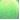
\includegraphics[width=3cm]{buoyimage}
    \caption{Cropped buoy}
    \label{fig:Cropped buoy for training data}
\end{figure}

\section{Gaussian Mixture Models and Maximum Likelihood Algorithm}
\subsection{Expectation Maximization Algorithm:}
EM algoritm is used for clustering the data in this case clustering and detecting yellow, orange and green buoys. We used 1-D gaussian distributions for each buoy which provided the distribution of dominant channel of the RGB colour space for that buoy. For green buoy, green channel is considered. For yellow channel Red + Green channel is considered. For orange channel, R channel is considered for gaussian distribution.

\begin{figure}[h]
    \centering
    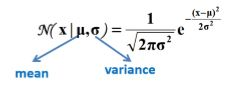
\includegraphics[width=6cm]{formula}
    \caption{1-D Gaussian Distribution formula}
    \label{fig:1-D Gaussian Distribution formula}
\end{figure}
\begin{figure}[h]
    \centering
    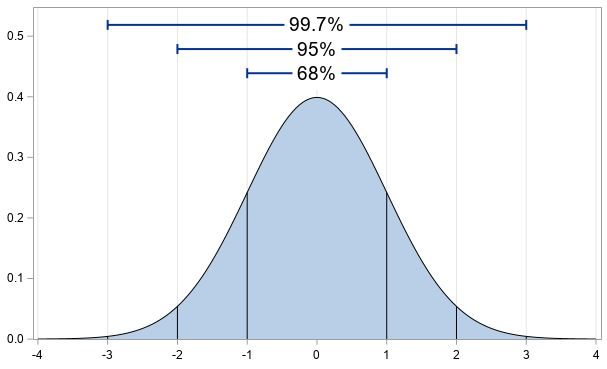
\includegraphics[width=5.2cm]{guassian}
    \caption{1-D Gaussian Distribution}
    \label{fig:1-D Gaussian Distribution}
\end{figure}

These are the steps involved in EM agoritm.
\begin{enumerate}
\item First step is to initialize mean and standard deviation with random values.
\item Then gaussian distribution is generated by passing data of R or G or B channel of colour space with the  randomized means and variances. 
\item E step: Then gaussian distibutions are combined along with their weightage. Weightage depends on number of clusters considered.
\begin{figure}[h]
    \centering
    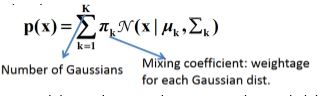
\includegraphics[width=9cm]{Estep}
    \caption{Combining gaussian Distributions}
    \label{fig:Combining gaussian Distributions}
\end{figure}
Then, the probabilities that the points belongs to a cluster must be found. This is found by using the formula:
\begin{figure}[h]
    \centering
    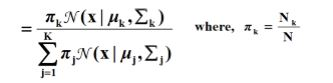
\includegraphics[width=9cm]{Pcx}
    \caption{Probability of the cluster given points}
    \label{fig:Probability of the cluster given points}
\end{figure}
\item M step: Now find the updated mean and standard deviation using the following formula:
\begin{figure}[h]
    \centering
    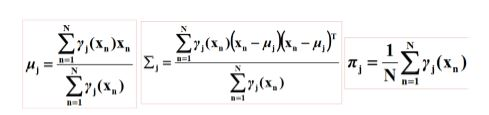
\includegraphics[width=9cm]{msd}
    \caption{Updated mean and SD formula}
    \label{fig:Updated mean and SD formula}
\end{figure}

\item Now we compute the log likelihood of the probabilitilies. This process is iterated until the difference between the consecutive log likelihoods is less than a threshold value.
\newpage
\begin{figure}[h]
    \centering
    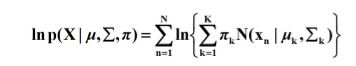
\includegraphics[width=9cm]{logl}
    \caption{Loglikelihood formula}
    \label{fig:Loglikelihood formula}
\end{figure}
\end{enumerate}
First the EM algorithm is tested before the traning step. This is done by creating a guassian distribution with known means and standard distributions and comparing the means and standard distribution obtained from the output of EM algorithm.
\newline
We have considered three guassian distributions of numbers randomly generated having means 0, 3, 6 and standard deviations 2, 0.5, 3. We have provided these data to put EM  algorithm and the following results are obrained. The means and standard deviations obtained from the EM algoritm are almost equal to the actual values.
\newline
 \begin{figure}[h]
    \centering
    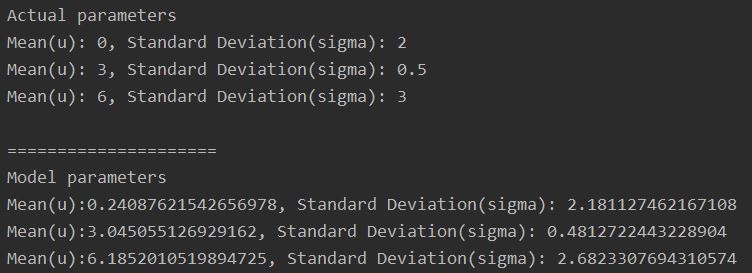
\includegraphics[width=13cm]{testoutput}
    \caption{Test output}
    \label{fig:Test output}
\end{figure}

\section{Learning Color Models}
In this section, we applied the process to our training data. But, before that we need compute and visualize the color histogram for each channel of the sampled/cropped images gathered during the data preparation phase for each image.This will provide some intuition on how many Gaussians [N] to fit to the color histogram. The following are the histogram outputs:
\newpage
\begin{figure}[h]
    \centering
    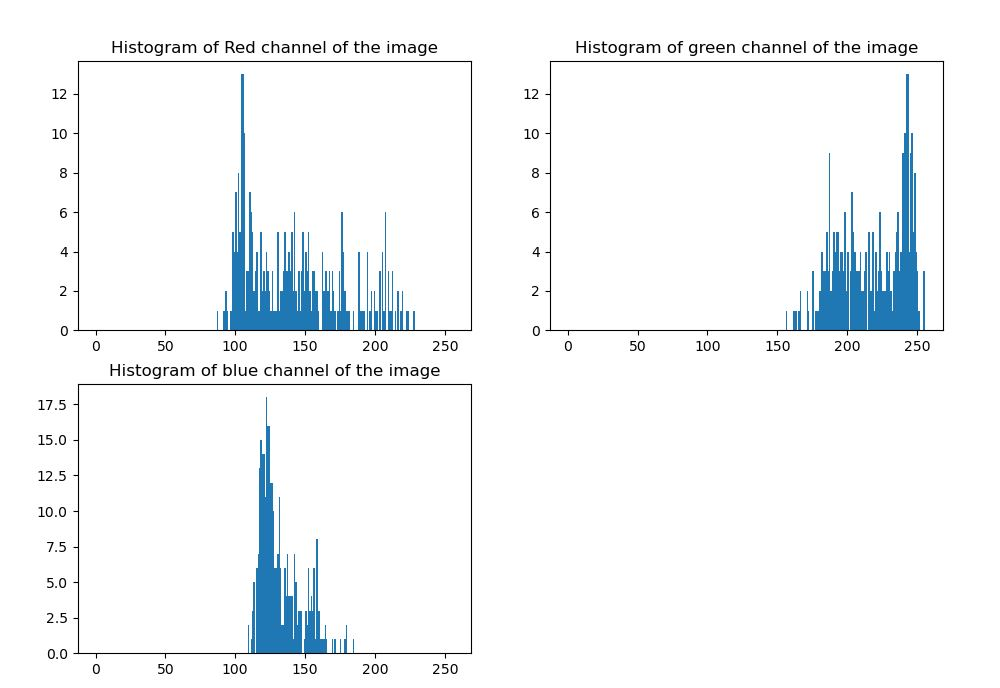
\includegraphics[width=13cm]{greenbuoyhistogram}
    \caption{Green buoy channel distribution}
    \label{fig:Green buoy channel distribution}
\end{figure}
For green buoy detection, 3 clusters are considered as there are three clusters formed in the Green channel distribution.
\newline
\begin{figure}[h]
    \centering
    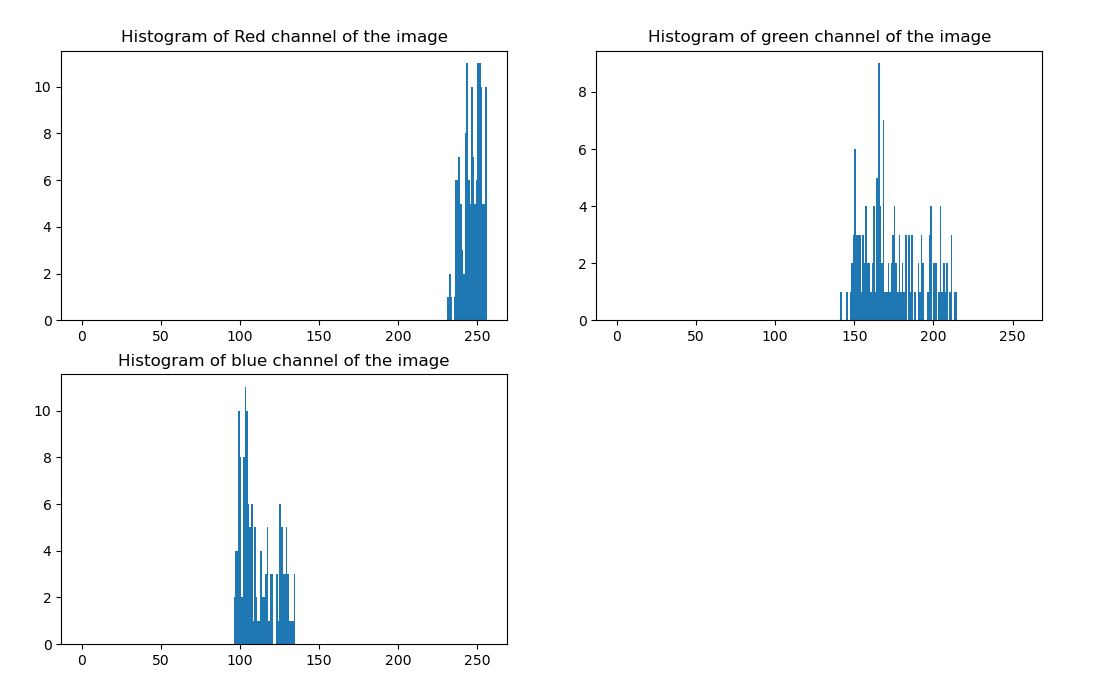
\includegraphics[width=13cm]{orangebuoyhistogram}
    \caption{Orange buoy channel distribution}
    \label{fig:Orange buoy channel distribution}
\end{figure}
\newline
For orange buoy detection, 2 clusters are considered as there are two clusters formed in the Red channel distribution.
\newpage
\begin{figure}[h]
    \centering
    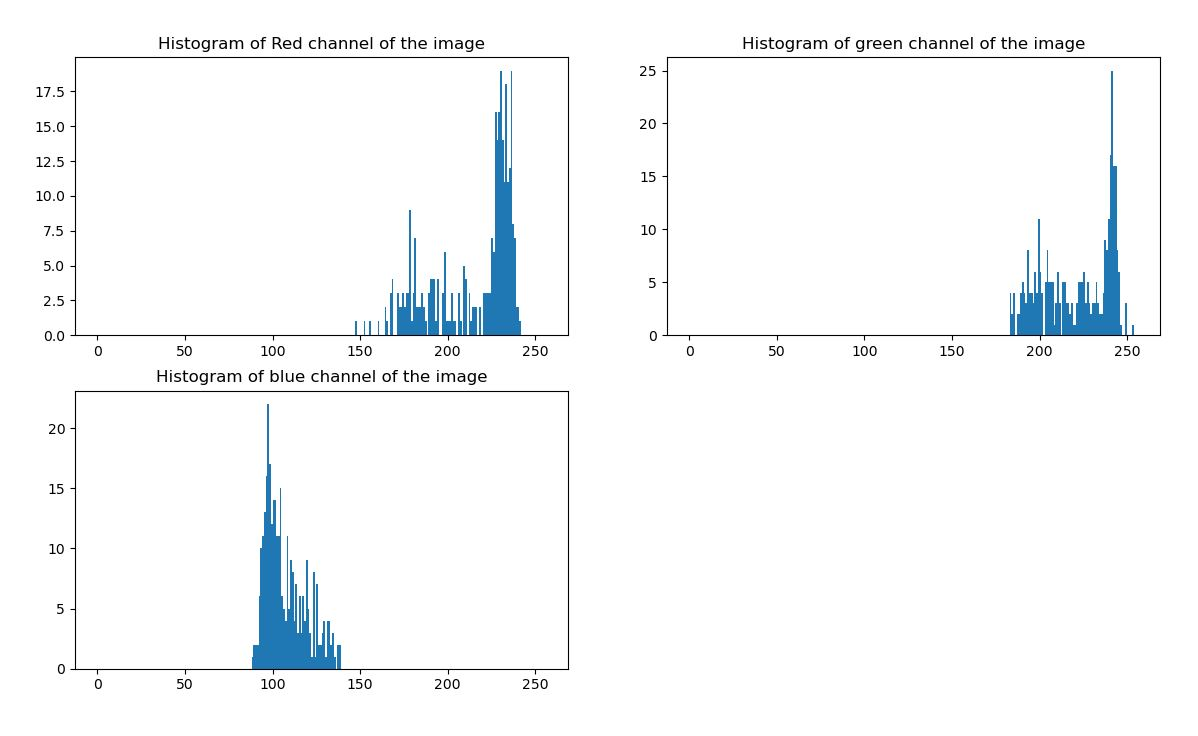
\includegraphics[width=15cm]{yellowbuoyhistogram}
    \caption{Yellow buoy channel distribution}
    \label{fig:Yellow buoy channel distribution}
\end{figure}
For yellow buoy detection, 2 clusters are considered as there are two major clusters formed each in  Red and Green channel distribution.

\section{Buoy Detection}
The following procedure is followed to detect the buoy:
\begin{enumerate}
\item First training and testing is performed on the obtained cropped images of the buoy in the Data preparation phase. We extract the channel of the image we want to work with as our data. As number of clusters are obtained from the histograms, we run the EM algoritm. The algorithm runs until it converges to the given value (bound = 0.0001) or until it reaches the maximum number of iterations specified (1000). For each cluster, the last mean and standard deviations are stored. 

\item Now the given input video is processed frame by frame. The same procedure is employed for frames. The data now becomes the channels of the frame we want to with. For 1-D gaussian distribution, the means and standard distributions obtained from training data is considered. Then again the probabilities are calculated for each pixel in the image. If the probabilities are grater than a threshold value, that channel of the pixel is made 255.

\item Then, the frame is blurred and edges are determined using canny edge detection.

\item Then, contours are found using $findcontours()$ function and only the contour with minimum length is considered as the buoy is small. Then we obtain the boundary points of the contours using $convexHull()$ function. 

\item Then, we enclose the hull with a circle using $cv2.Circle()$ function. 
\end{enumerate}
\newpage
\section{Output}
The following are the output frames obtained after detecting the buoys:
\begin{figure}[h]
    \centering
    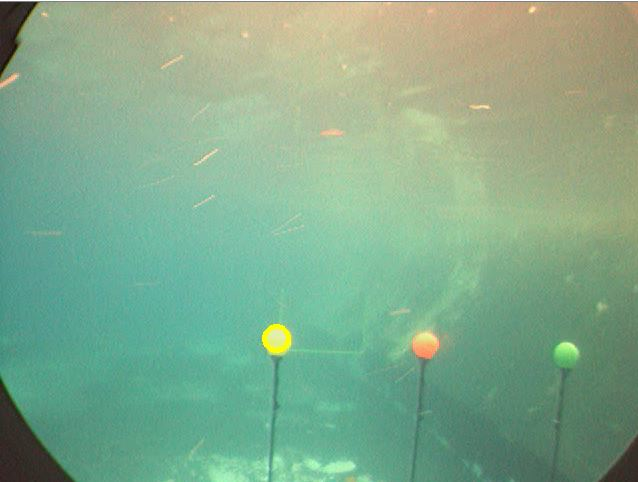
\includegraphics[width=16cm]{yellowbuoydetection}
    \caption{Yellow buoy detection}
    \label{fig:Yellow buoy detection}
\end{figure}
\newpage
\begin{figure}[h]
    \centering
    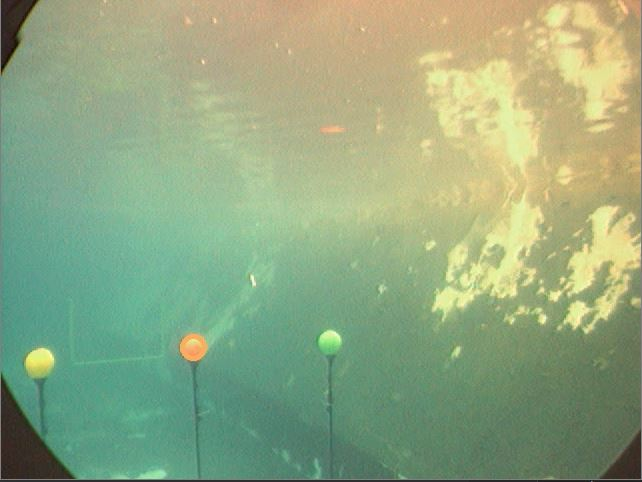
\includegraphics[width=16cm]{orangebuoydetection}
    \caption{Orange buoy detection}
    \label{fig:Orange buoy detection}
\end{figure}
\newpage
\begin{figure}[h]
    \centering
    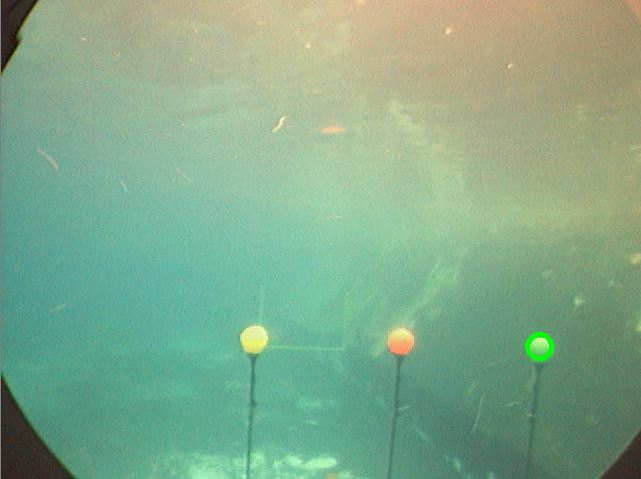
\includegraphics[width=16cm]{greenbuoydetection}
    \caption{Green buoy detection}
    \label{fig:Green buoy detection}
\end{figure}

\section{Challenges Faced:}
Detection of green buoy was very difficult as the video has only few frames containing green buoy.
\section{Team Members:}
1. Eashwar Sathyamurthy
2. Akwasi A Obeng
3. Achal P Vyas
\section{Output Videos:}
To access output videos please use this \href{https://drive.google.com/drive/folders/1u-9GdSQYNw-M6Cw1d2jZkYR8QPCDGkzQ?usp=sharing}{\underline{link}}.
\end{document}
